\chapter{Material e Métodos}\label{database}

A partir da base de dados do Projeto SOS-CHUVA, cinco casos foram selecionados, onde houve queda de granizo medida pela rede de \textit{hailpads} (\autoref{hailpads}). A \autoref{tabela_casos} mostra uma breve descrição de cada caso.

\begin{table}[htb]
	\IBGEtab{%
		\caption{Descrição dos casos selecionados para análise.}%
		\label{tabela_casos}
	}{%
		\begin{tabularx}{\textwidth}{cYYY}
			\toprule
			Caso & Descrição & Regiões Afetadas & Tipo de Severidade \\
			\midrule
			2016-12-25 & Condições instáveis na região levou à formação de diversos sistemas convectivos & Campinas, Vale do Paraíba, São Carlos & Rajadas de vento, granizo \\
			\midrule 
			2017-01-31 & Linha de Instabilidade & Sorocaba, Itu, Araraquara & Granizo \\
			\midrule 
			2017-03-14 & Chuva forte e queda de granizo entre Campinas e Indaiatuba e em Jacareí & Campinas, Indaiatuba, Jacareí & Granizo \\
			\midrule 
			2017-11-15 & Condições termodinâmicas favoráveis levaram à formação de sistemas convectivos concentrados no centro do estado de SP & Indaiatuba, Bebedouro & Granizo \\
			\midrule 
			2017-11-16 & Condições termodinâmicas favoráveis e um cavado em médios níveis favoreceram a formação de sistemas convectivos & Lorena, Ribeirão Preto, Campinas, São Paulo, Itapeva & Rajadas de vento, granizo \\
			\bottomrule
		\end{tabularx}%
	}{%
		\fonte{Adaptado de https://topicssoschuva.blogspot.com.br/2017/03/summary-of-case-studies.html.}%
	}
\end{table}


\section{Rede de Detecção de Granizo}\label{hailpads}

Dentro do Projeto SOS-CHUVA, uma rede de detecção de granizo foi instalada na Região Metropolitana de Campinas, dentro da cobertura do radar meteorológico Banda-X instalado na UNICAMP (XPOL). Como mostrado na Figura\autoref{rede_hailpads}, a rede foi composta por 24 localidades, com maior densidade de pontos nas cidades de Campinas e Indaiatuba. O instrumento, chamado de \textit{hailpad}, é composto por uma placa de isopor usado para isolamento coberta por uma folha de alumínio e fixada em um suporte de ferro aproximadamente 1,5 m acima da superfície. A primeira versão desse instrumento foi desenvolvida por \citeonline{Schleusener1960a} e \citeonline{ Decker1961}. Na Figura\autoref{hailpad_indaiatuba} é possível observar uma placa instalada em Indaiatuba.

\begin{figure}[htb]
	\begin{center}
		\caption{(a) Rede de \textit{hailpads} instalada na Região Metropolitana de Campinas com a localização e cobertura de 80 km do radar XPOL. (b) Hailpad instalado na cidade de Indaiatuba, na localização indicada com a seta em (a)} 
		\label{overview_hailpads}
		\subfloat[]{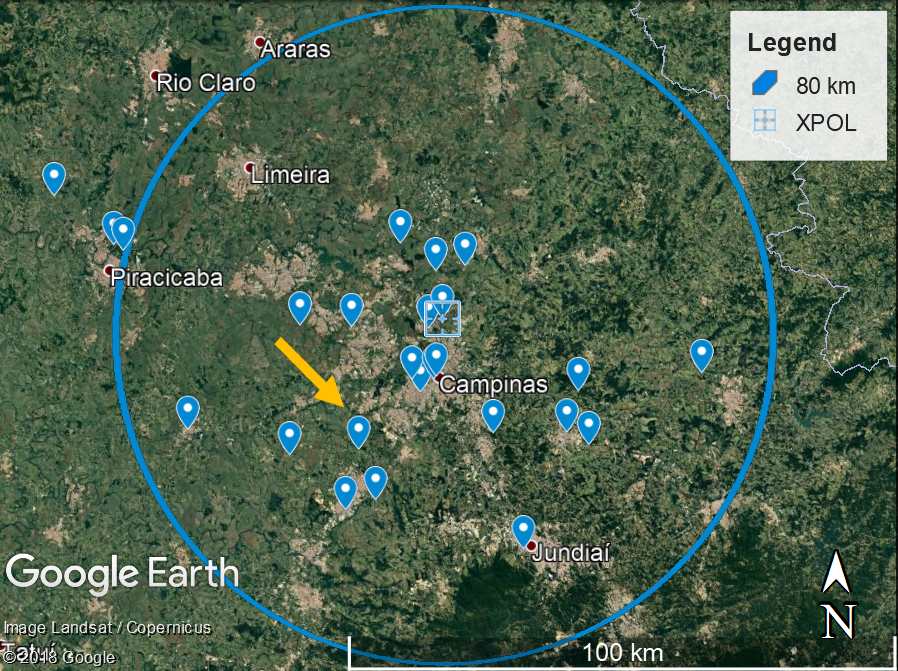
\includegraphics[width=0.75\columnwidth]{figs/hailpad_network.png}
			\label{rede_hailpads}}
		\ \
		\subfloat[]{\includegraphics[width=0.158\columnwidth]{figs/hailpad.png}
			\label{hailpad_indaiatuba}}\\
		\legend{Fonte: Produzido pela autora.}
	\end{center}
\end{figure}

Os casos descritos na \autoref{tabela_casos} foram selecionados com base nos registros dos \textit{hailpads} dentro da rede. A \autoref{tabela_hailpads} mostra a localização das placas e os grupos que mediram a distribuição de tamanho de granizo, sendo eles: Departamento de Ciências Atmosféricas (DCA/IAG-USP) e Laboratório de Instrumentação Meteorológica (LIM/CPTEC-INPE). Não houve registro da localização exata da placa C004. 

\begin{table}[htb]
	\IBGEtab{%
		\caption{Descrição dos \textit{hailpads} coletados para cada caso}%
		\label{tabela_hailpads}
	}{%
		\begin{tabularx}{\textwidth}{YYYY}
			\toprule
			Data do evento & Código do \textit{hailpad} coletado & Localização & Medido por \\
			\midrule 
			2016-12-25 & C002 & Campinas & IAG, LIM \\
			\midrule 
			2017-01-31 & C003 & Campinas & IAG, LIM \\ 
			 & C004 & Arredores de Campinas & IAG, LIM \\
			\midrule 
			2017-03-14 & C001 & Cosmópolis & IAG \\ 
			& R002 & Indaiatuba & IAG \\
			\midrule 
			2017-11-15 & R004 & Indaiatuba & IAG \\
			\midrule 
			2017-11-16 & R038 & Campinas & IAG \\
			\bottomrule
		\end{tabularx}%
	}{%
		\fonte{Produzido pela autora.}%
	}
\end{table}

A partir de um \textit{hailpad} é possível derivar diversas grandezas relacionadas à tempestade que gerou a queda de granizo. A principal delas é a distribuição de tamanho de granizo, medindo as cavidades na placa sensibilizada (\autoref{hailpad_exemplo}). Essa grandeza foi obtida através de uma série de medições manuais dos diâmetros das cavidades com um paquímetro e ajustando os dados com a curva de calibração desse tipo de isopor, realizada pelo LIM e exibida na \autoref{calibracao_hailpad}. Com essa distribuição, pode-se calcular a energia cinética do granizo (quando diversas placas mediram um mesmo evento) ou do \textit{hailpad} (quando poucas ou uma única placa mediram um evento). Ambas grandezas são equivalentes ao trabalho mecânico sofrido pela superfície onde caiu o granizo, indicando então o dano causado por ele na superfície.

\begin{figure}[htb]
	\begin{center}
		\caption{Placa R004 sensibilizada no sítio (a) e sem a cobertura de alumínio (b)} 
		\label{hailpad_exemplo}
		\subfloat[]{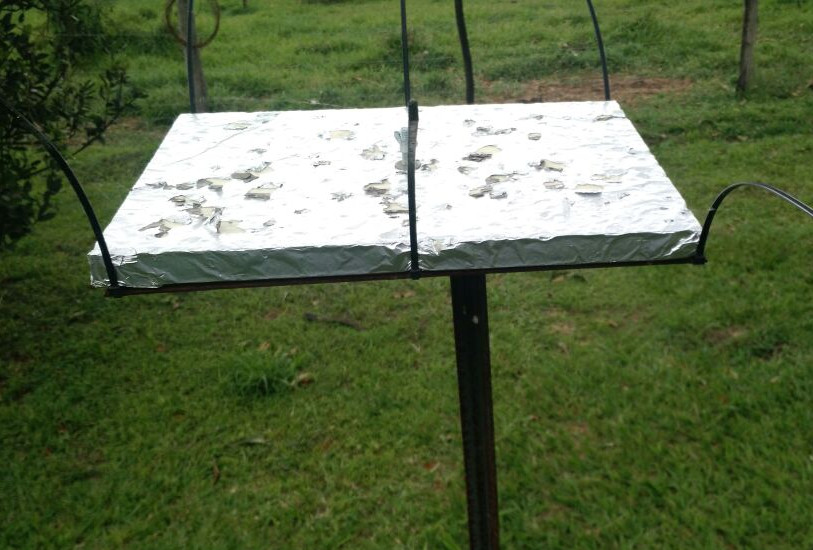
\includegraphics[width=0.4\columnwidth]{figs/hailpad_site.jpg}
			\label{hailpad_sensibilizado}}
		\quad
		\subfloat[]{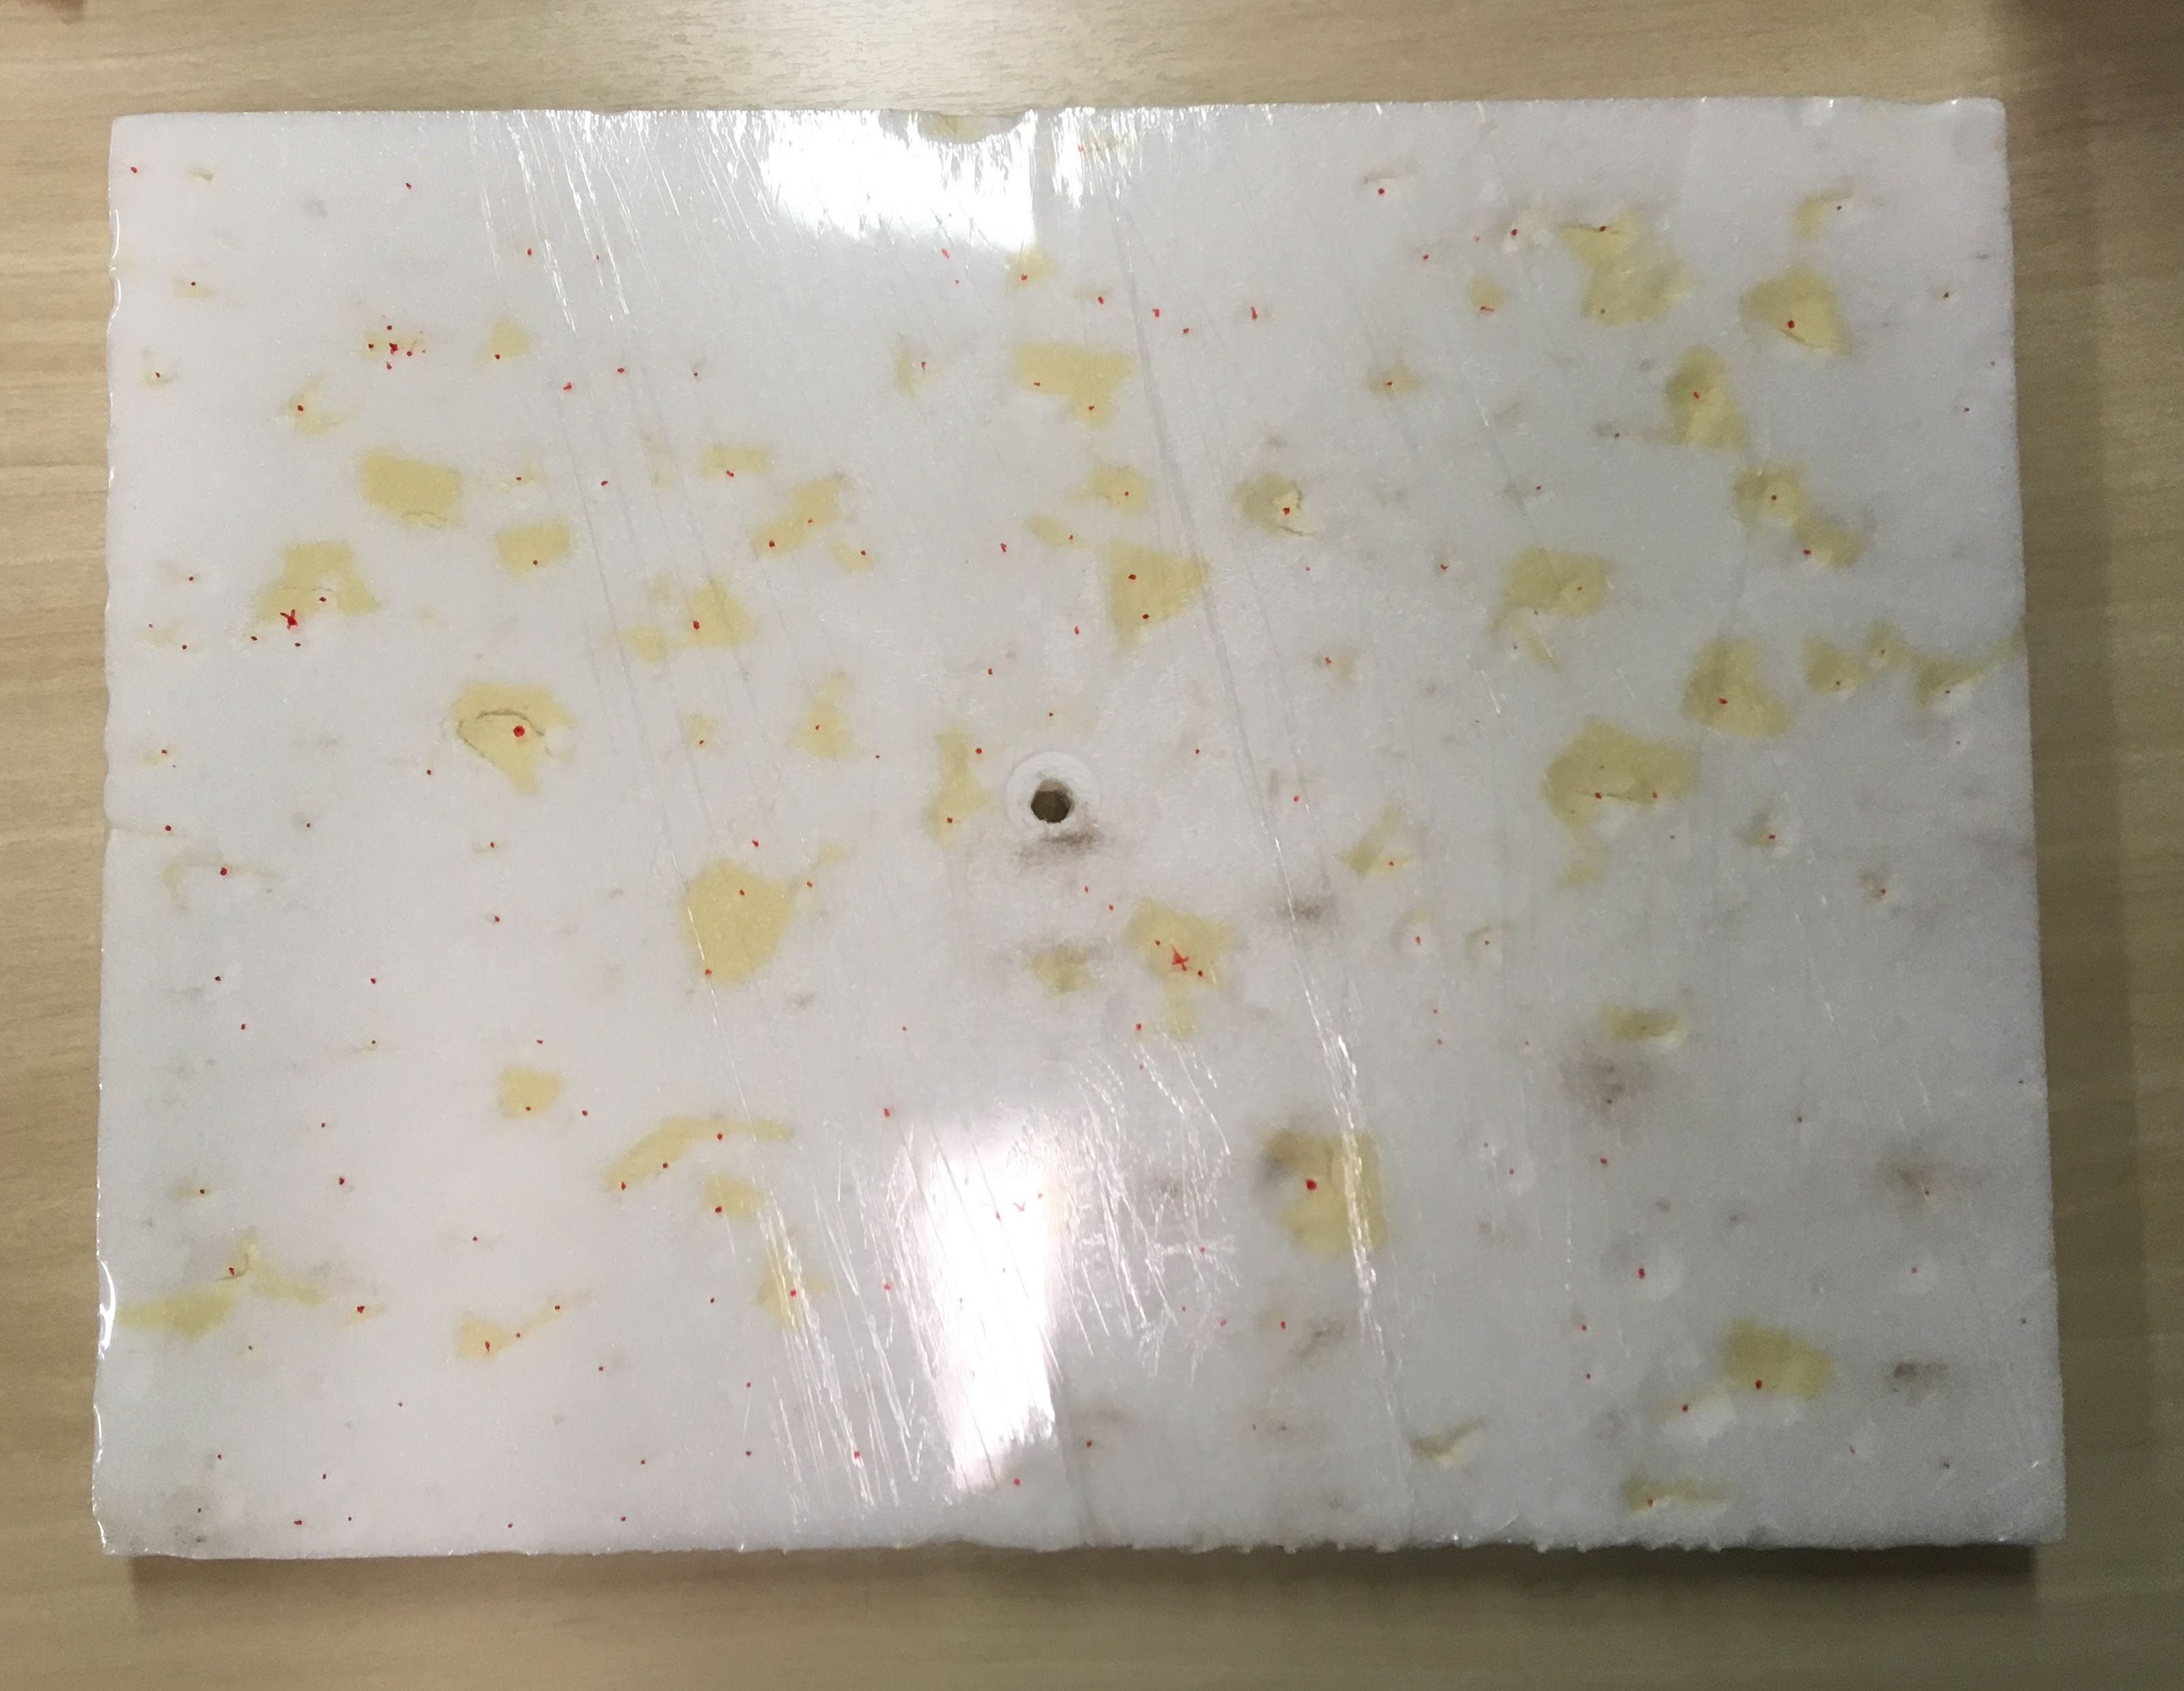
\includegraphics[width=0.355\columnwidth]{figs/hailpad_used.JPG}
			\label{hailpad_semaluminio}}\\
		\legend{Fonte: A autora.}
	\end{center}
\end{figure}

\begin{figure}[htb]
	\begin{center}
		\caption{Curva de calibração do \textit{hailpad} obtida pelo LIM/CPTEC-INPE} 
		\label{calibracao_hailpad}
%		\setcaptionmargin{1cm}
		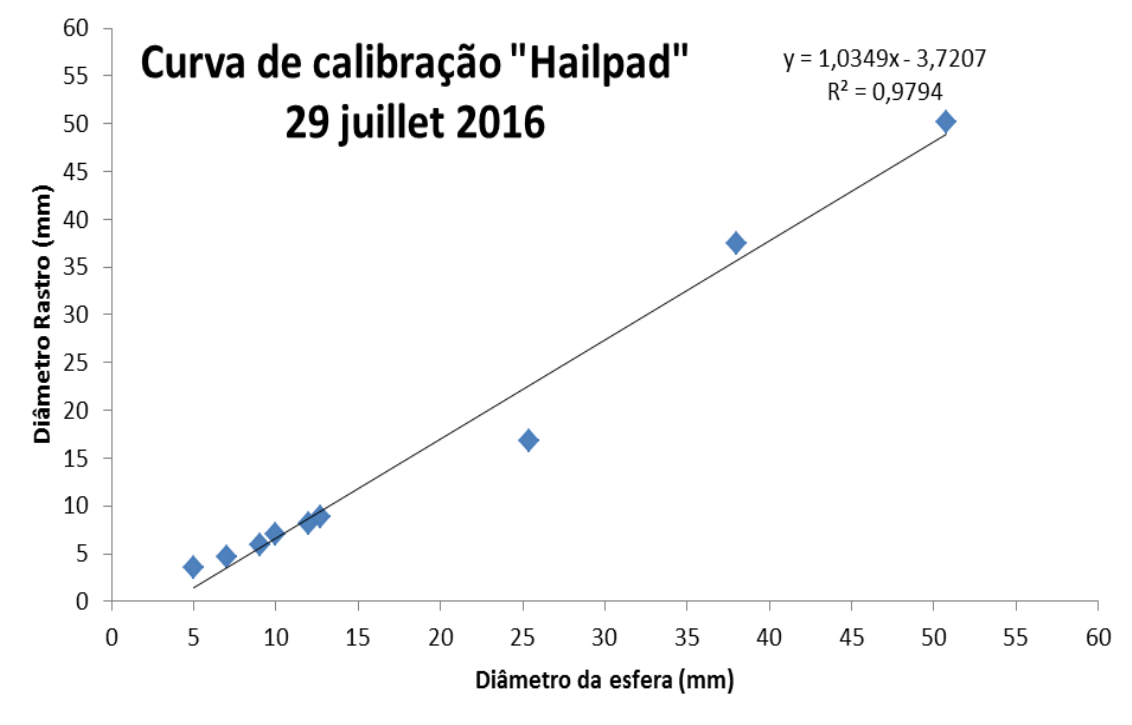
\includegraphics[width=0.7\columnwidth]{figs/calibracao_hailpad.png}
		\legend{Fonte: \citeonline{ThomazJunior2015a}.}
	\end{center}
\end{figure}

Como houve no máximo 2 placas sensibilizadas em todos os casos, calculou-se a energia cinética do \textit{hailpad} $E_t\:(Jm^{-2})$, definida por \citeonline{Mezeix1981} como:

\begin{equation} \label{mezeix}
	E_t = 4,58\:e^{-6} \sum_{i=1}^{k} n_i d_i^4
\end{equation}

\noindent
sendo $n_i$ a quantidade de pontos por $m^2$ em um dado diâmetro médio $d_i\:(mm)$ de um intervalo $\Delta d$. $k$ é o numero de intervalos, igual a 9 nesse caso já que $\Delta d$ variou entre $2$ e $22\:\:mm$ com espaçamento de $1\:mm$. Foram consideradas incertezas nas medidas propagando o desvio-padrão da distribuição média entre as diferentes medidas de uma mesma placa.

Com os valores de diâmetro do granizo e energia cinética do \textit{hailpad}, duas escalas que definem a intensidade de tempestades de granizo foram comparadas entre si. A \autoref{tabela_escalas} descreve as escalas ANELFA e TORRO, comparando-as de acordo com o descrito por \citeonline{Dessens2007}. A escala ANELFA, referente à organização que a desenvolveu (\textit{Association Nationale d'Etude et de Lutte contre les Fléaux Atmosphériques}, Associação para Suprimir Pragas Atmosféricas), foi desenvolvida na França usando uma série de 16 anos de dados de \textit{hailpads} e compara o diâmetro máximo do granizo com a energia cinética do \textit{hailpad}, indicando possíveis danos (principalmente a plantações) que um evento com dado tamanho de granizo pode causar \cite{Dessens2007}. O índice varia entre A0 (onde ocorre danos à folhas de árvores) e A5 (onde o evento é extremamente perigoso e pode causar mortes). A escala TORRO de intensidade de queda de granizo, também referente à organização que a desenvolveu (\textit{Tornado and Storm Research Organisation}, Organização de Pesquisa em Tornado e Tempestade), foi desenvolvida na Grã-Bretanha e compara o diâmetro típico (interpretado aqui como a mediana da distribuição) do granizo com a energia cinética e também indica possíveis danos que o evento pode causar \cite{webb1986}. Este índice varia entre H0 (onde não há danos) e H10 (onde há extensivos danos estruturais).

\begin{table}[hp]
	\IBGEtab{%
		\caption{Descrição das escalas ANELFA e TORRO, com comparação entre o dano típico de cada escala.}%
		\label{tabela_escalas}
	}{%
		\begin{tabularx}{\textwidth}{YcYcY}
			\toprule
			 & \multicolumn{2}{c}{ANELFA} & \multicolumn{2}{c}{TORRO} \\
			\midrule
			Objeto Equivalente ao Tamanho do Granizo & Escala & Dano Típico & Escala & Dano Típico \\
			\midrule
			Ervilha & A0 & Acidentes de trânsito, danos a folhas de árvores & H0 & Sem danos
\\
			\midrule 
			Naftalina & A1 & Danos a vinhas, pomares, tabaco & H1 & Danos gerais leves a plantas e plantações
 \\
			\midrule 
			Bola de Gude, Uva & A2 & Danos sérios a cereais, vegetais, árvores & H2 & Danos significativos a frutas, plantações e vegetações
\\
			\midrule 
			Noz & A3 & Danos totais a todas as plantações, vidros quebrados, carros danificados & H3 & Danos severos a frutas e plantações, danos a estruturas de vidro e plástico, pinturas em madeiras
\\
			\midrule 
			Ovo de Pombo a Bola de Squash & A4 & Paisagem de inverno, mortes de animais, pessoas feridas, danos a aviões pousados & H4 & Danos difundidos em vidros, danos em carrocerias de veículos
\\
			Bola de Golfe a Ovo de Franga & & & H5 & Destruição total de vidros, danos a telhados de azulejo, riscos significativos de ferimentos
\\
			\midrule 
			Ovo de Galinha & A5 & Evento extremamente perigoso, morte de pessoas desprotegidas & H6 & Carrocerias de aeronaves pousadas amassadas, paredes de tijolos furadas
\\
			Bola de Tênis a Bola de Cricket & & & H7 & Danos severos a telhados, risco de ferimentos sérios
\\
			Laranja Grande a Bola de Softball & & & H8 & (Evento mais severo registrado nas Ilhas Britânicas) Danos severos a aeronaves
\\
			Toranja & & & H9 & Danos estruturais extensivos; Risco de ferimentos severos ou até fatais em pessoas a céu aberto
\\
			Melão & & & H10 & Danos estruturais extensivos; Risco de ferimentos severos ou até fatais em pessoas a céu aberto \\
			\bottomrule
		\end{tabularx}%
	}{%
		\fonte{Adaptado de \citeonline{Dessens2007} e \url{http://www.torro.org.uk/hscale.php}.}%
	}
\end{table}


\section{Radares Meteorológicos}\label{radar}

A \autoref{cobertura_radares} mostra a localização e cobertura espacial dos radares utilizados neste trabalho. A \autoref{estrategia_radares} mostra a estratégia de varredura de cada radar.

\begin{figure}[htb]
	\begin{center}
		\caption{Localização e cobertura dos radares da FCTH (laranja), de São Roque (azul) e o XPOL (verde). As linhas mais grossas representam a cobertura de $250$ ($80$) $km$ dos radares FCTH e São Roque (XPOL), enquanto que as linhas mais finas representam a cobertura de $100$ ($60$) $km$ dos mesmos radares} 
		\label{cobertura_radares}
		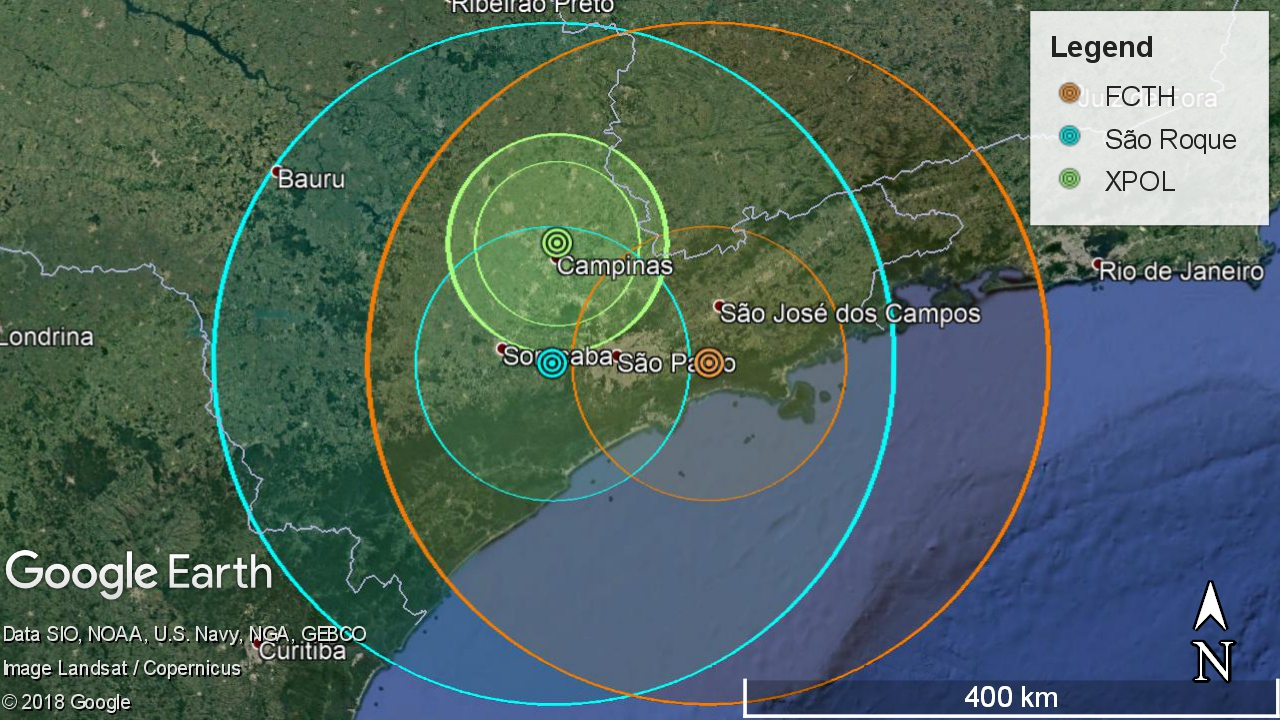
\includegraphics[width=\columnwidth]{figs/radar_coverages_hires2.jpg}
		\legend{Fonte: Produzido pela autora.}
	\end{center}
\end{figure}

O radar Doppler Banda-S de dupla polarização operado pela Fundação Centro Tecnológico de Hidráulica (FCTH) é localizado na barragem de Ponte Nova, município de Biritiba Mirim (\ang{23;36;}\:S, \ang{45;58;20}\:W, $916\:m$ de altitude). Este radar faz uma varredura volumétrica a cada 5 minutos em uma cobertura de até $250\:km$, com 8 elevações (\ang{1}, \ang{1,6}, \ang{2,4}, \ang{3,2}, \ang{4,2}, \ang{5,5}, \ang{6,9} e \ang{8,6}) de \ang{1} de abertura do feixe, como mostra a Figura\autoref{estrategia_cth}. A velocidade de Nyquist (valor máximo (mínimo no caso negativo) de velocidade radial medido) deste radar é de $16,27\:ms^{-1}$. Os dados volumétricos foram convertidos em uma grade de $1\:x\:1\:x\:1\:km$ usando o pacote Py-ART (\textit{Python ARM Radar Toolkit}, Conjunto de Ferramentas de Radar em Python do ARM) \cite{Helmus2016} e perfis horizontais (em $3\:km$ de altura) e verticais (cortes entre dois pontos com coordenadas latitudinais e longitudinais) foram analisados. Além da variável refletividade do radar (medida em $dBZ$), três variáveis polarimétricas foram analisadas e relacionadas com diferentes tipos de hidrometeoros seguindo a classificação de \citeonline{Straka2000} descrita na \autoref{hid}:

\begin{alineas}
	\item \textbf{Refletividade Diferencial ($dBZ$)}: Razão entre os fatores de refletividade horizontal e verticalmente polarizados; diferencia a forma das partículas em um dado volume medido;
	\item \textbf{Fase Diferencial Específica ($^\circ\:km^{-1}$)}: Calculada a partir das matrizes de espalhamento vertical e horizontal, é fortemente influenciada pela concentração numérica e massa de gotículas de nuvem, permitindo a derivação da distribuição de tamanho das mesmas;
	\item \textbf{Coeficiente de Correlação (adimensional)}: Razão entre as amplitudes das matrizes de espalhamento; destaca misturas de formas e tamanhos das partículas \cite{Rauber2018}.
\end{alineas}

O radar Doppler Banda-S operado pelo DECEA (Departamento de Controle do Espaço Aéreo) instalado em São Roque (\ang{23;35;56}\:S, \ang{47;5;52}\:W, $1147,54\:m$ de altitude) faz varreduras a cada 10 minutos em uma cobertura de até $250\:km$, com 15 elevações (\ang{0,5}, \ang{1}, \ang{2}, \ang{3}, \ang{4}, \ang{5}, \ang{6}, \ang{7}, \ang{8}, \ang{9}, \ang{10}, \ang{12}, \ang{14}, \ang{16} e \ang{18}) de \ang{2} de abertura do feixe, como mostra a Figura\autoref{estrategia_sr}. A velocidade de Nyquist deste radar é de $14,63\:ms^{-1}$. Os perfis horizontais de CAPPIs (\textit{Constant Altitude Plan Position Indicator}, Indicador Plano de Posição em Altitude Constante) em $3\:km$ de altura serviram como dados de entrada para o algoritmo ForTraCC (\textit{Forecast and Tracking the Evolution of Cloud Clusters}, Prevendo e Rastreando a Evolução de Aglomerados de Nuvens) \cite{Vila2008} adaptado para radares meteorológicos. Este algoritmo identifica os sistemas convectivos usando um limiar de refletividade - $35\:dBZ$ neste trabalho - e os classifica usando imagens subsequentes: sistema novo (\textit{new}), em continuidade (\textit{continuity}), em fusão (\textit{merge}) ou em separação (\textit{split}) - A \autoref{fortracc_teoria} mostra uma ilustração dessas situações.

\begin{figure}[htb]
	\begin{center}
		\caption{Representação dos tipos de classificação do ForTraCC: continuidade (a), separação (b) e fusão (c). As formas com contorno pontilhado representa o sistema no primeiro passo enquanto que as formas cinzas representam o sistema no passo seguinte, com as setas indicando o deslocamento} 
		\label{fortracc_teoria}
		%		\setcaptionmargin{1cm}
		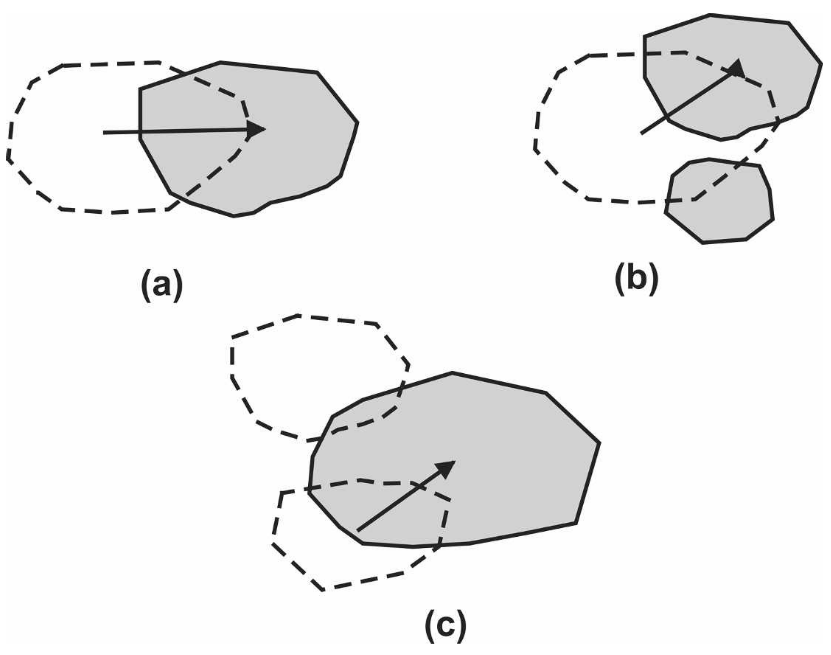
\includegraphics[width=0.5\columnwidth]{figs/fortracc_classes.png}
		\legend{Fonte: \citeonline{Vila2008}.}
	\end{center}
\end{figure}

O ciclo de vida da tempestade associada a cada caso foi definido a partir do sistema convectivo com maior intensidade na posição do \textit{hailpad}, considerando o horário aproximado da queda de granizo. A partir desse sistema, a família - definição do algoritmo para um conjunto de sistemas próximos uns aos outros com mesmo deslocamento - associada a ele foi extraída e corrigida caso houvesse necessidade. A partir de cada rastreamento, variáveis como refletividade máxima e tamanho do sistema foram analisadas, além de servirem como base para a seleção de descargas elétricas associadas aos sistemas.

O radar Doppler Banda-X de dupla polarização XPOL foi operado pelo Projeto SOS-CHUVA na UNICAMP, cidade de Campinas (\ang{22;48;50}\:S, \ang{47;3;22}\:W, $680\:m$ de altitude). Ele fez varreduras volumétricas a cada 10 minutos em uma cobertura de até $80\:km$, com 17 elevações (\ang{0,5}, \ang{1,8}, \ang{3,1}, \ang{4,4}, \ang{5,7}, \ang{7}, \ang{8,3}, \ang{9,6}, \ang{10,9}, \ang{13}, \ang{15}, \ang{18}, \ang{22}, \ang{26}, \ang{32}, \ang{40} e \ang{55}) de \ang{1,3} de abertura do feixe, como mostra a Figura\autoref{estrategia_xpol}. Por ser de uma banda de frequência mais alta, a velocidade de Nyquist deste radar é menor do que a dos radares Banda-S: $9,6\:ms^{-1}$. Os dados volumétricos também foram convertidos em uma grade de $1\:x\:1\:x\:1\:km$ e as variáveis refletividade do radar e velocidade radial foram utilizadas. Devido à falta de dados em muitos dos casos selecionados, este radar foi usado apenas como entrada no algoritmo de recuperação de vento por Multi-Doppler (\autoref{multidoppler}) juntamente com os demais radares.

\begin{figure}[hp]
	\begin{center}
		\caption{Estratégia de varredura volumétrica dos radares meteorológicos da FCTH (a), de São Roque (b) e o XPOL instalado na UNICAMP (c)} 
		\label{estrategia_radares}
		\subfloat[]{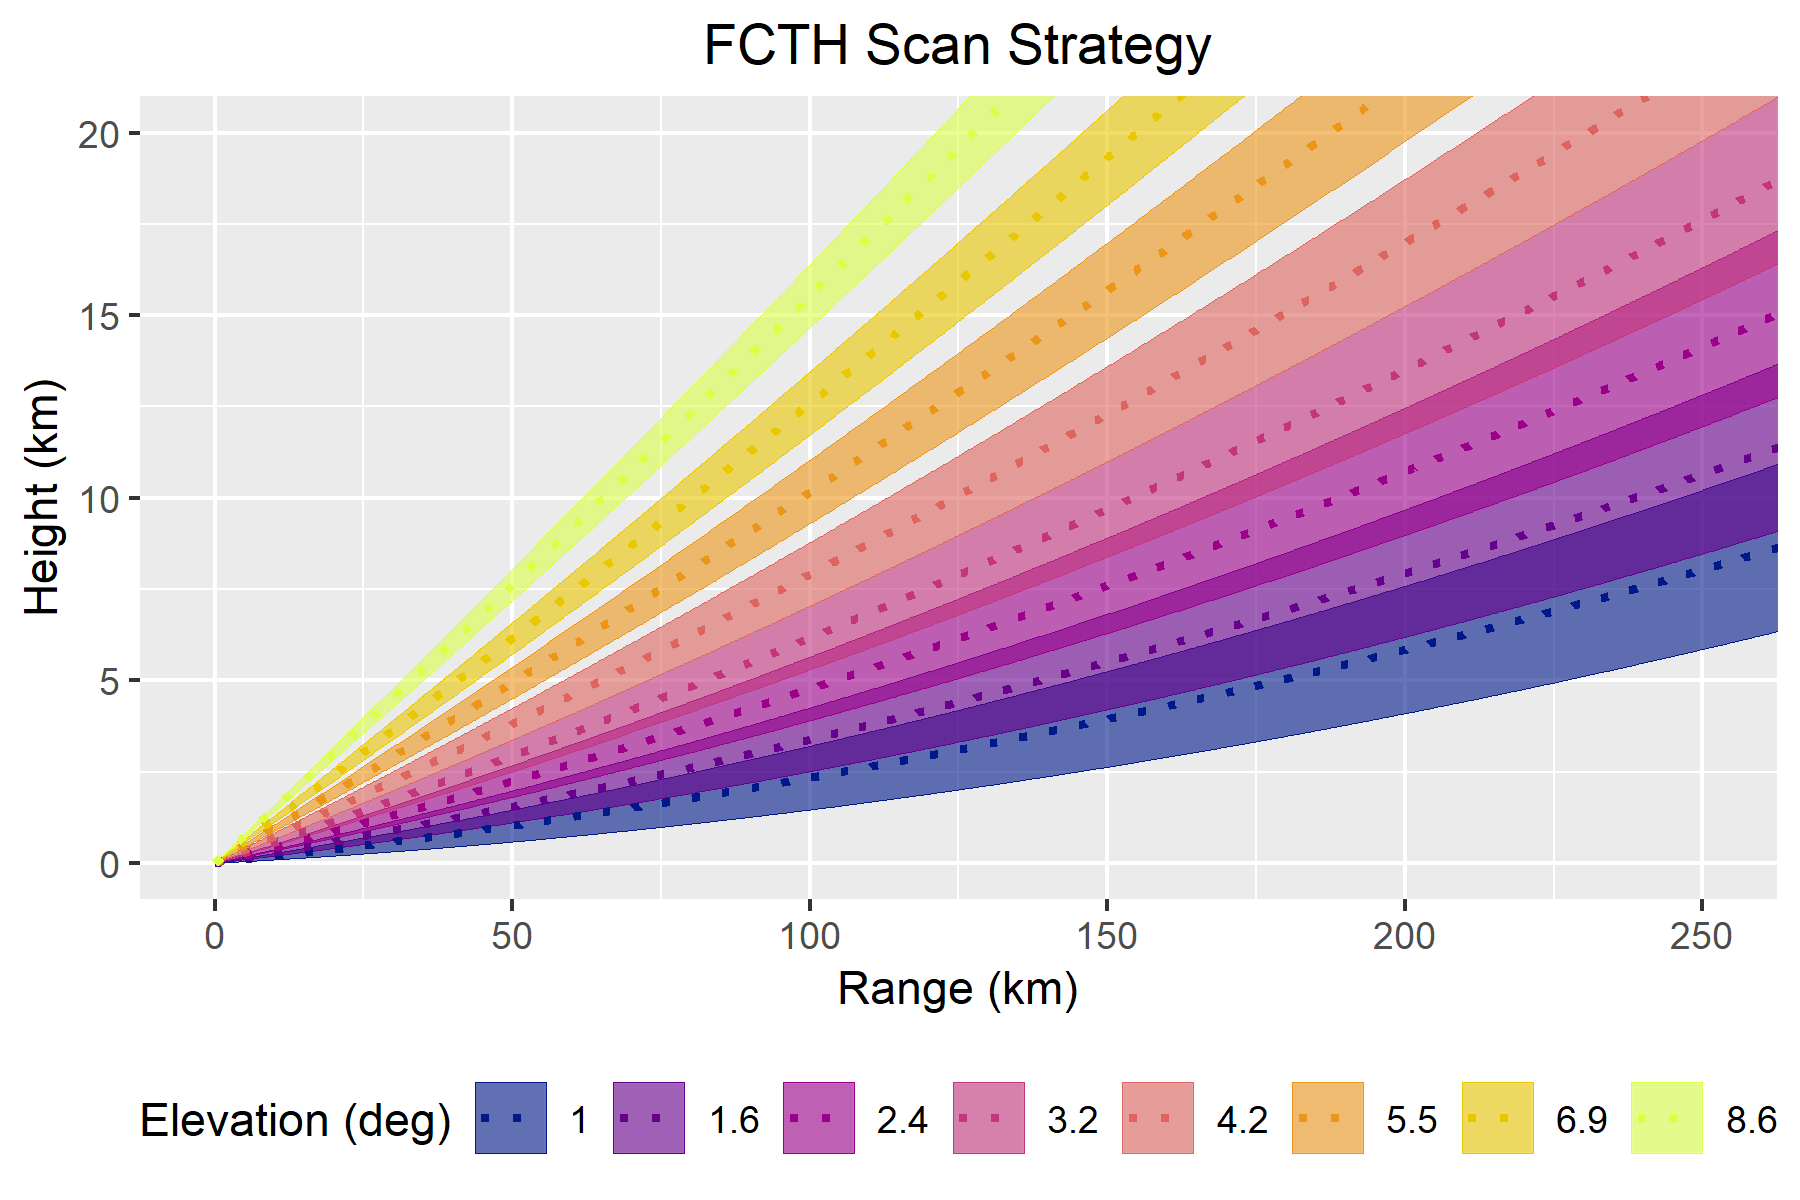
\includegraphics[width=0.75\columnwidth]{../General_Processing/figures/scan_strategy_cth.png}\label{estrategia_cth}}\\
		\subfloat[]{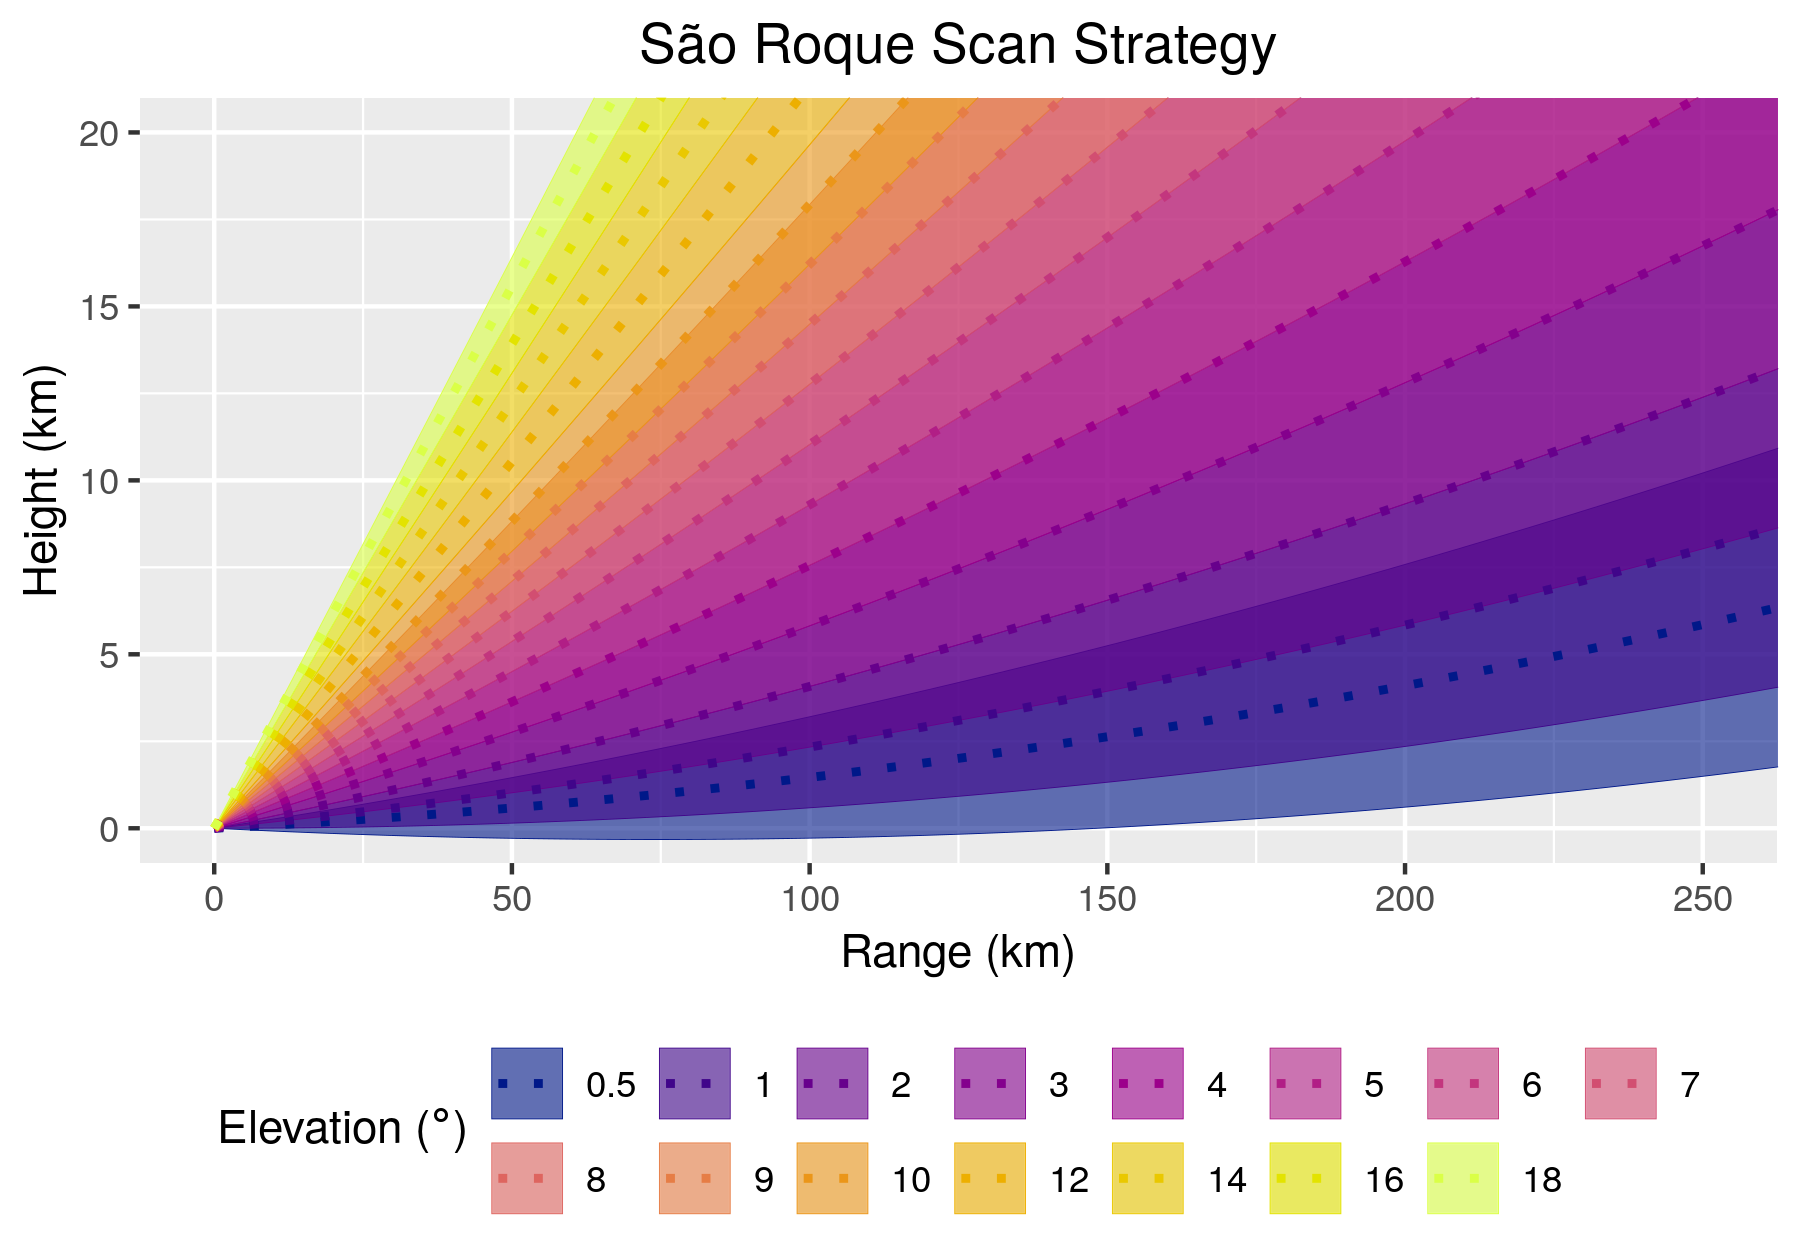
\includegraphics[width=0.75\columnwidth]{../General_Processing/figures/scan_strategy_sr.png}\label{estrategia_sr}}\\
		\subfloat[]{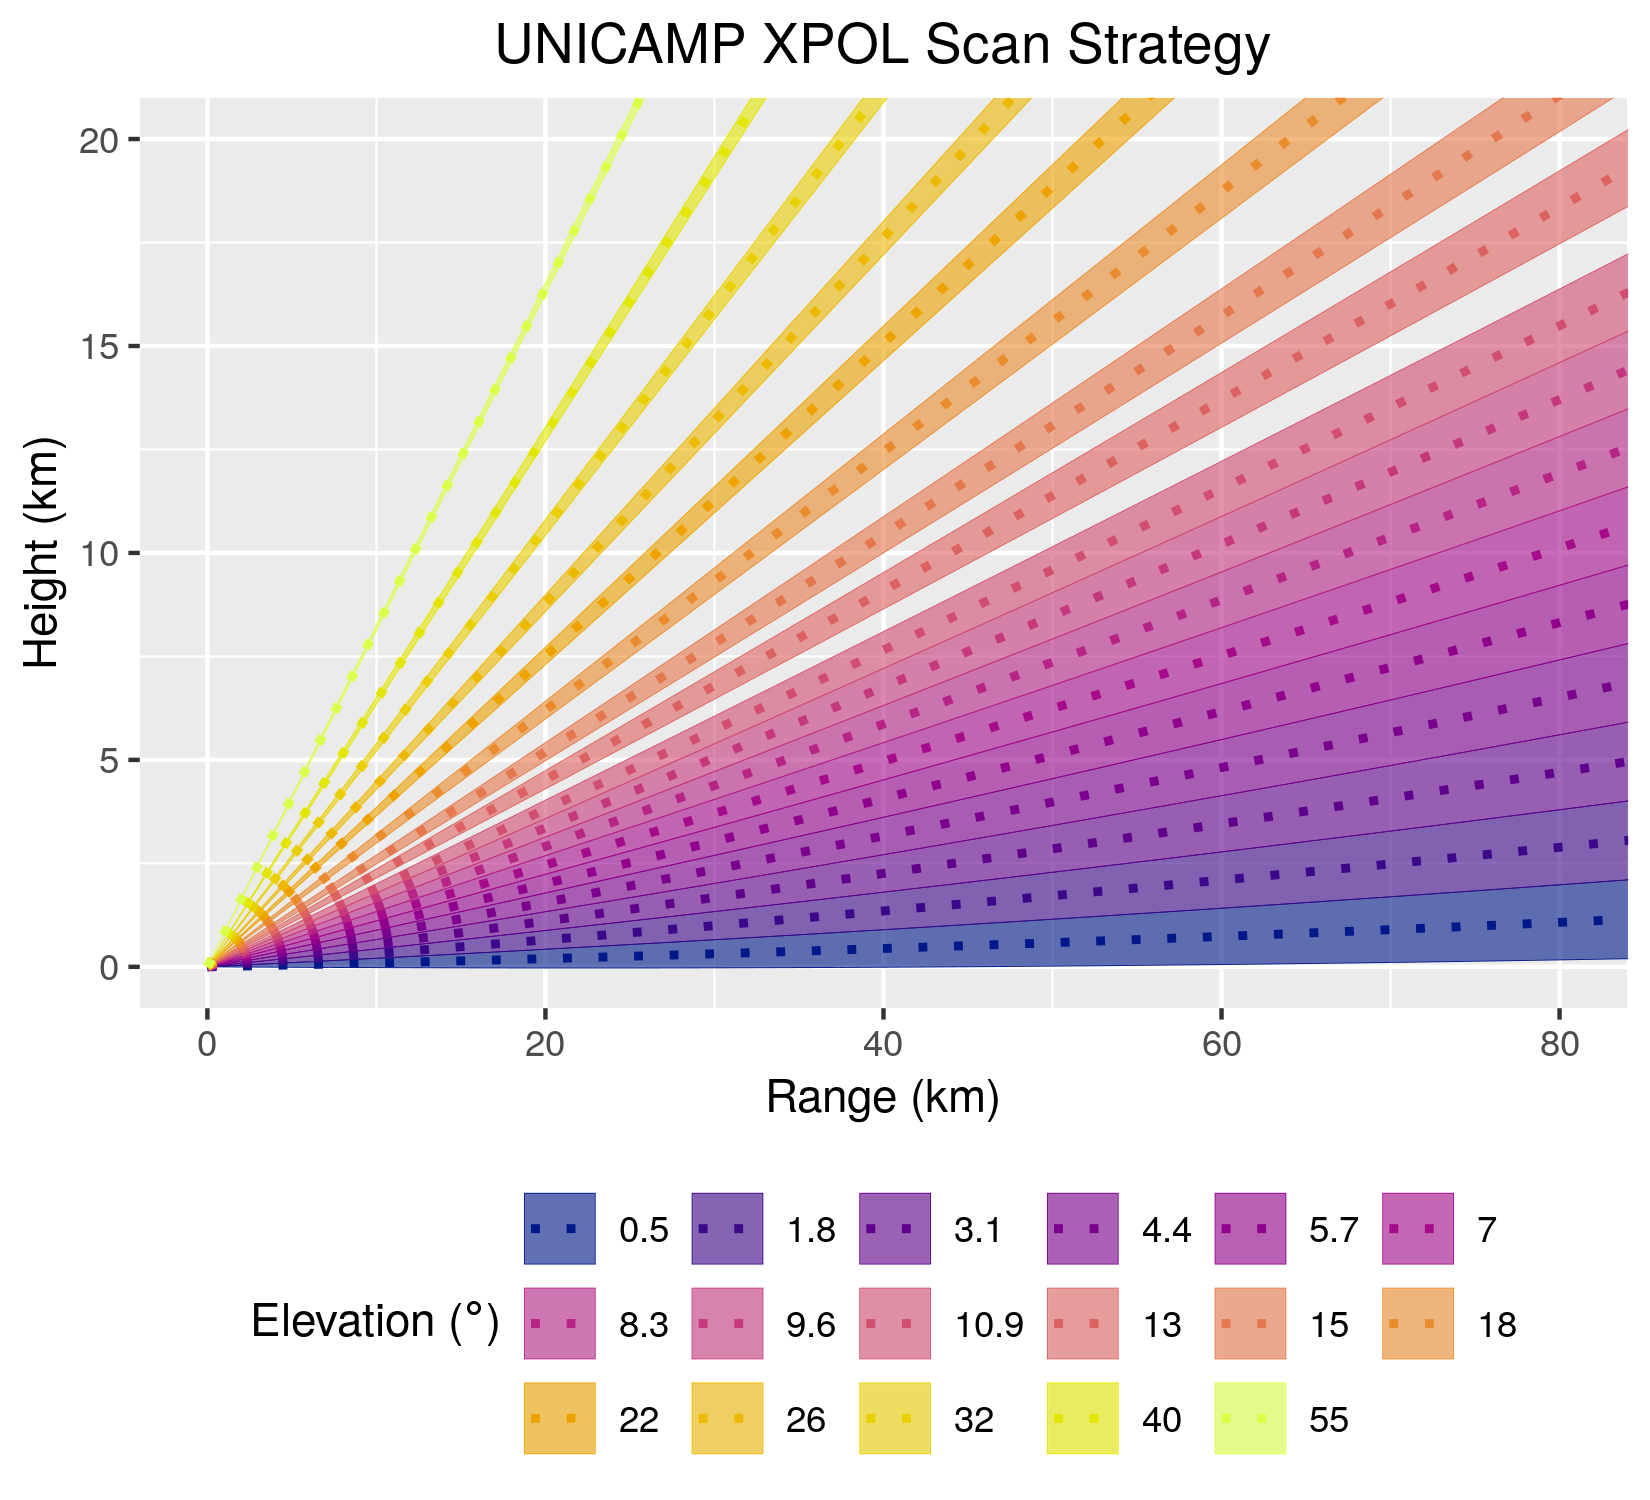
\includegraphics[width=0.75\columnwidth]{../General_Processing/figures/scan_strategy_xpol.png}\label{estrategia_xpol}}\\
		\legend{Fonte: Produzido pela autora.}
	\end{center}
\end{figure}

\subsection{Identificação de Hidrometeoros}\label{hid}

Para definir de forma mais acurada a presença de granizo nas medidas de radar, o método de classificação de hidrometeoros usando Lógica Fuzzy foi aplicado. Presente no pacote CSU\_RadarTools \cite{Lang2017a} através de uma função chamada \textit{Fuzzy Hydrometeor Classificator} (Classificador Fuzzy de Hidrometeoros), o método implementado é dividido em três passos:

\begin{alineas}
	\item A \textbf{fuzzificação} usa funções beta, que indicam a probabilidade de um dado valor de variável polarimétrica representar um dado tipo de hidrometeoro, com pesos específicos para cada variável (refletividade e temperatura apresentam o maior peso) para classificar os dados polarimétricos de entrada em cada ponto de grade;
	\item A \textbf{inferência} calcula uma pontuação para cada tipo de hidrometeoro somando as classificações de cada variável e;
	\item A \textbf{agregação} escolhe a pontuação máxima para cada ponto e indica o hidrometeoro correspondente a ela \cite{Liu2000a}.
\end{alineas}

Esta função é aplicada em tempestades de verão e diferencia 10 tipos de hidrometeoros:

\begin{alineas}
	\item Chuvisco (\textit{Drizzle})
	\item Chuva (\textit{Rain})
	\item Cristais de Gelo (\textit{Ice Crystals})
	\item Agregados (\textit{Aggregates})
	\item Neve Molhada (\textit{Wet Snow})
	\item Gelo Vertical (\textit{Vertical Ice})
	\item Graupel de Densidade Baixa (\textit{Low-Density Graupel})
	\item Graupel de Densidade Alta (\textit{High-Density Graupel})
	\item Granizo (\textit{Hail})
	\item Gotas Grandes (\textit{Big Drops})
\end{alineas}

A função utiliza como entrada os campos de refletividade, refletividade diferencial, fase diferencial específica e coeficiente de correlação, além de um perfil de temperatura obtido a partir de uma radiossondagem. O método de cálculo utilizado (chamado de híbrido) não usa pesos fixos para a refletividade e perfil de temperatura, apenas para as variáveis polarimétricas: os pesos foram de 0,8 (refletividade diferencial), 1 (fase diferencial específica) e 0,8 (coeficiente de correlação). As radiossondagens aplicadas foram coletadas no Campo de Marte (Estação SBMT, São Paulo) em datas próximas aos eventos e os dados foram processados usando o pacote Siphon \cite{siphon}.

Para verificar subjetivamente a performance do método de classificação de hidrometeoros, os campos de variáveis polarimétricas foram analisados e relacionados com os mesmos tipos de hidrometeoros do método a partir da classificação de \citeonline{Straka2000}. A \autoref{hid_straka} mostra os intervalos de valores de cada variável correspondente a cada tipo de hidrometeoro, incluindo também a mistura de chuva com granizo (\textit{rain + hail}).

\begin{figure}[htb]
	\begin{center}
		\caption{Classificação de hidrometeoros de acordo com refletividade (a), refletividade diferencial (b), fase diferencial específica (c) e coeficiente de correlação (ou razão de correlação cruzada) (d)} 
		\label{hid_straka}
%		\setcaptionmargin{1cm}
		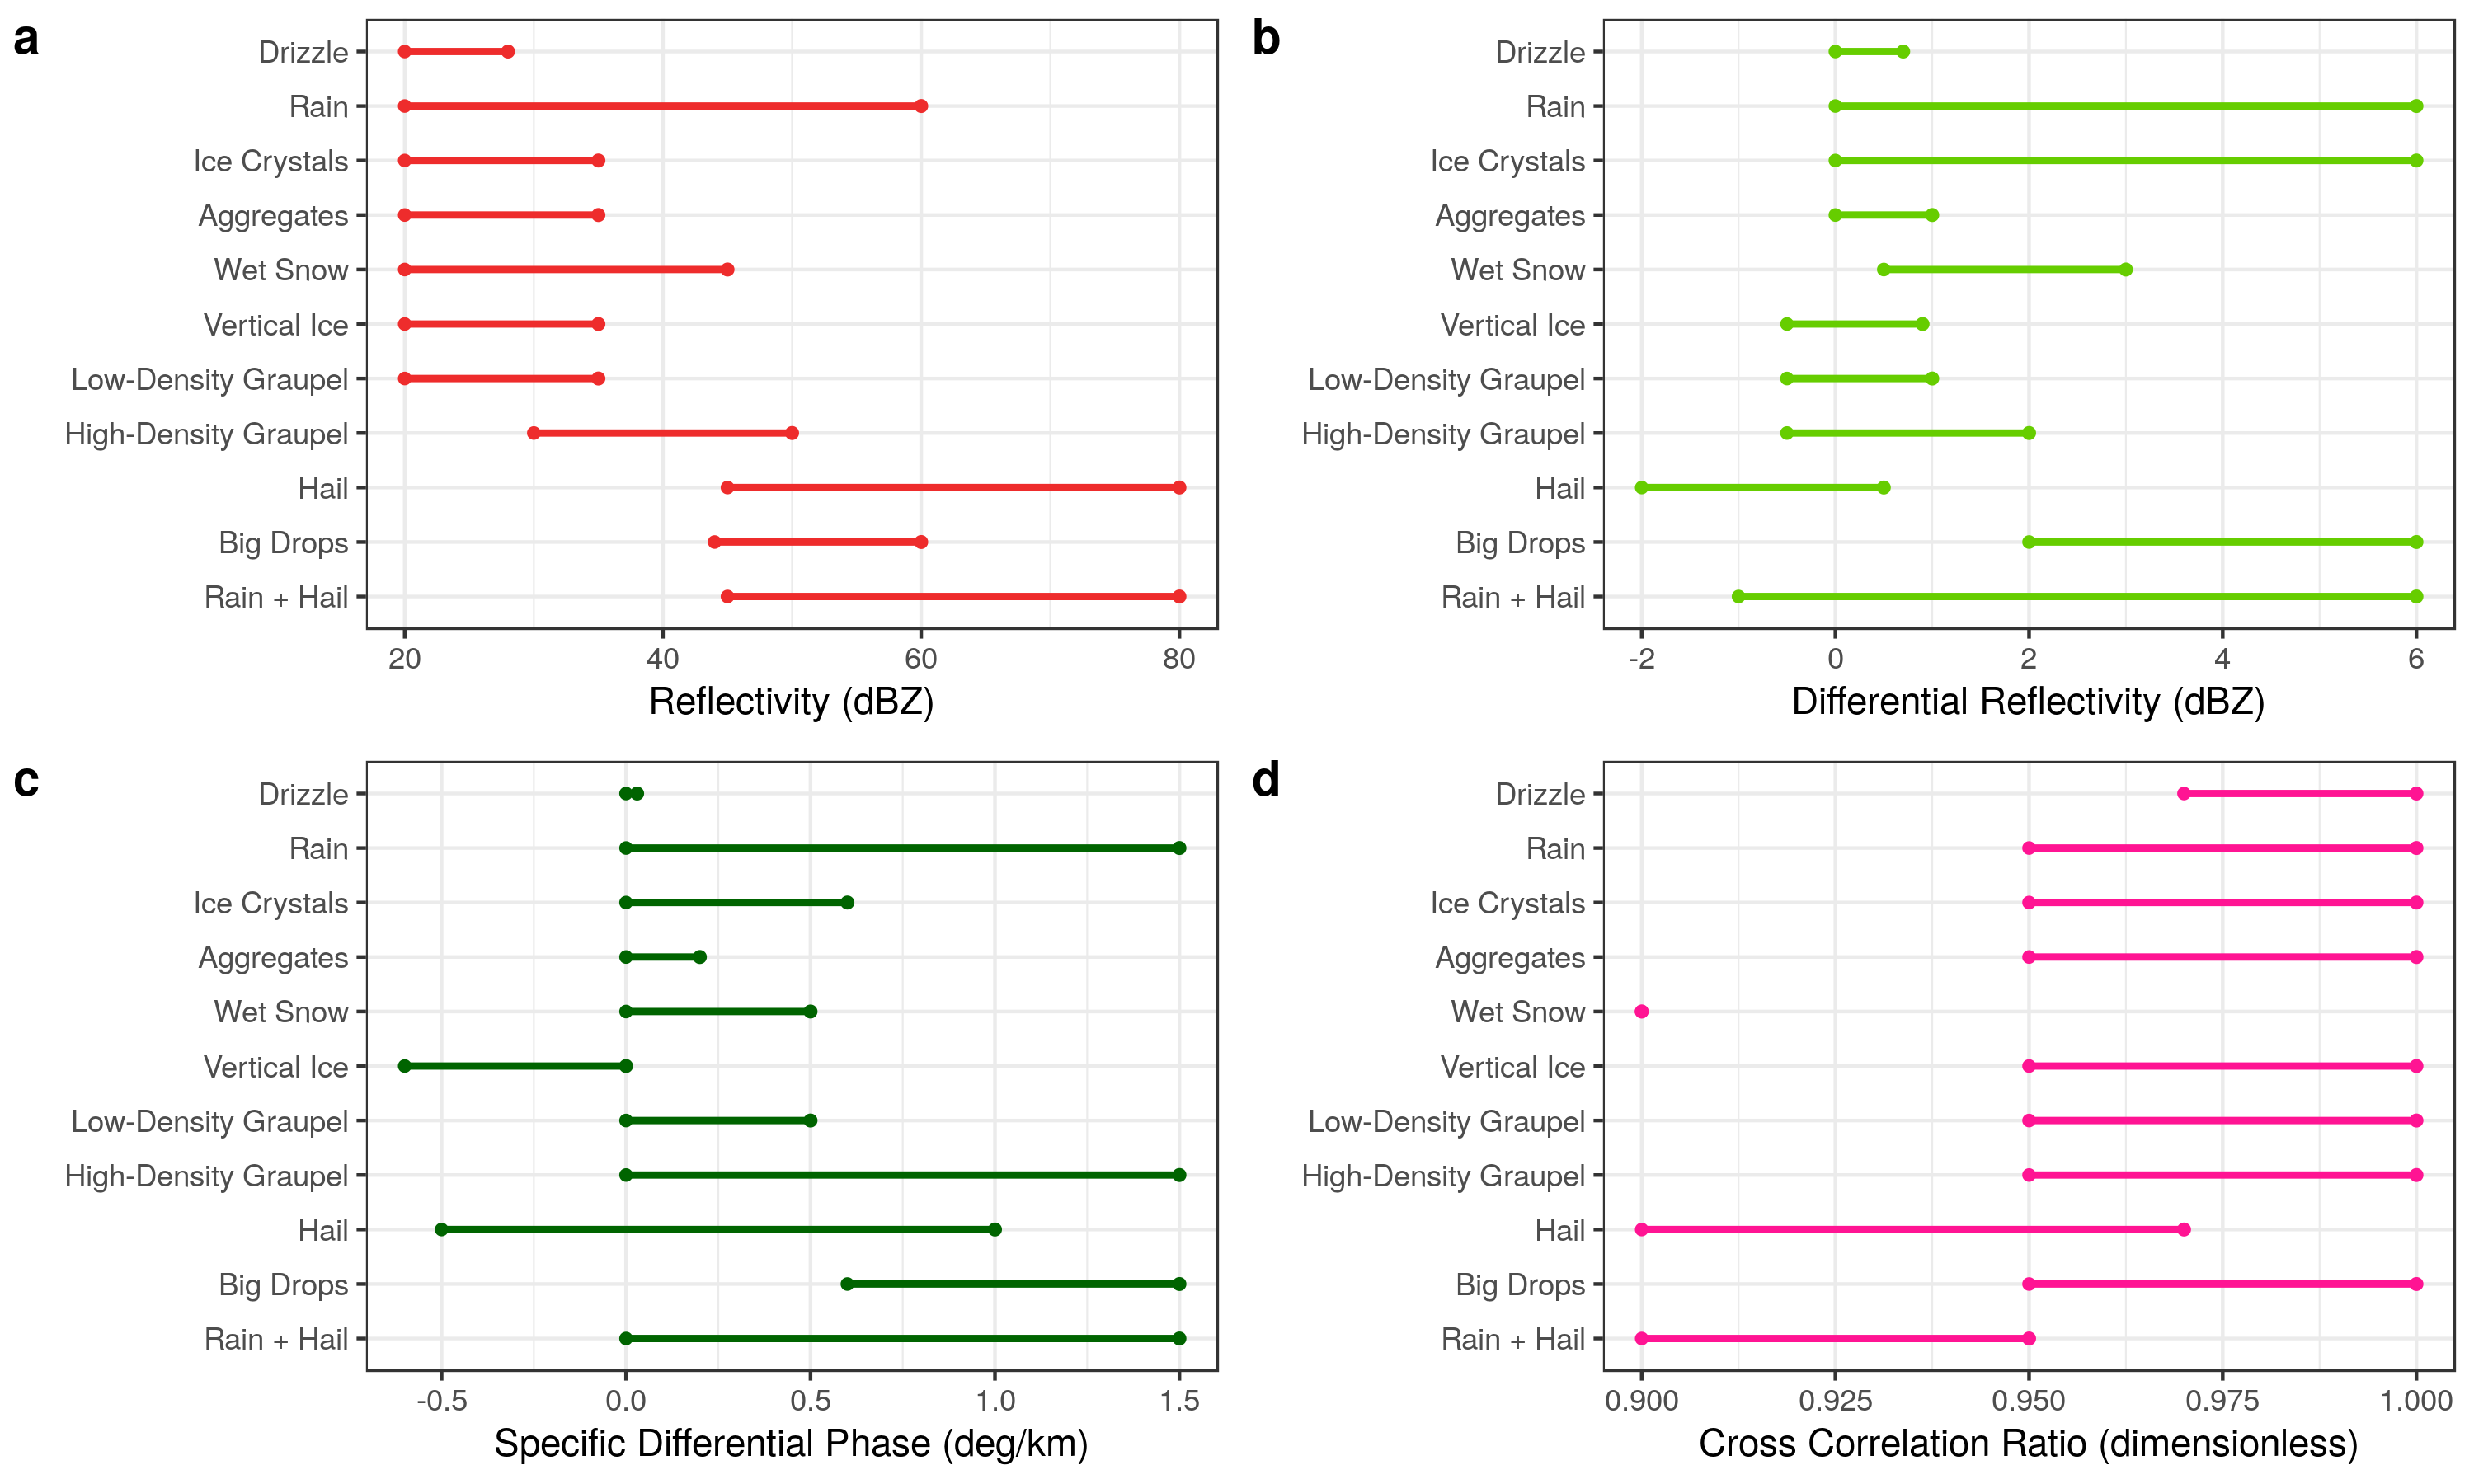
\includegraphics[width=\columnwidth]{../General_Processing/figures/hids_strakaetal.png}
		\legend{Fonte: Produzido pela autora a partir de \citeonline{Straka2000}.}
	\end{center}
\end{figure}

Outra função do pacote CSU\_RadarTools usada neste trabalho chama-se \textit{Liquid/Ice Water Mass Calculations} (Cálculos de Massas de Água Líquida e Gelo), que utiliza de entrada a refletividade e a refletividade diferencial. A partir do cálculo da contribuição da chuva para a refletividade horizontal - e consequentemente da contribuição do gelo através do resíduo da mesma - a massa de água líquida é derivada, usando a refletividade diferencial quando a água líquida é predominante. A massa de gelo é calculada apenas a partir da contribuição do gelo por uma aproximação de Rayleigh \cite{Carey2000, Cifelli2002b}.

\subsection{Recuperação de Vento por Multi-Doppler}\label{multidoppler}

A área de estudo possui cobertura de pelo menos dois radares - três se considerar a cobertura máxima dos radares (\autoref{cobertura_radares}) - capazes de medir velocidade radial (Doppler) quase simultaneamente (\autoref{tabela_radares_md}). Isso permite a aplicação de métodos que convertem os campos tridimensionais de refletividade e velocidade radial de múltiplas perspectivas em um campo tridimensional de velocidade do vento com alto grau de detalhamento.

\begin{table}[htb]
	\IBGEtab{%
		\caption{Configuração dos radares nos casos em que a recuperação de vento por Multi-Doppler foi utilizada}%
		\label{tabela_radares_md}
	}{%
		\begin{tabularx}{0.8\textwidth}{Yccccc}
			\toprule
			Caso & \multicolumn{2}{c}{2017-03-14} & \multicolumn{3}{c}{2017-11-15} \\
			\midrule 
			Radares disponíveis & FCTH & SR & FCTH & SR & XPOL \\
			\midrule 
			Resolução temporal ($s$) & $300$ & $600$ & $300$ & $600$ & $600$ \\ 
			\midrule 
			Diferença mínima entre os horários de começo da varredura dos radares ($s$) & \multicolumn{2}{c}{$172$} & \multicolumn{3}{c}{$19$} \\
			\midrule
			Diferença máxima entre os horários de começo da varredura dos radares ($s$) & \multicolumn{2}{c}{$174$} & \multicolumn{3}{c}{$20$} \\
			\bottomrule
		\end{tabularx}%
	}{%
		\fonte{Produzido pela autora.}%
	}
\end{table}

A \autoref{doppler_lobes} mostra o mesmo da \autoref{doppler_theory_lobes}, mas para combinações entre os três radares usados neste trabalho. Considerando a combinação FCTH/XPOL (painel superior), a distância entre os radares e a localização do XPOL dentro da cidade de Campinas limita as estimativas boas ou aceitáveis em boa parte da região de estudo, com exceção da cidade de Indaiatuba e à oeste dela. Considerando a combinação SR/FCTH (painel central), a estimativa Dual-Doppler tem erros menores (ou seja, $\beta=\ang{45}$) em Campinas e Indaiatuba (cidades com mais casos de queda de granizo, \autoref{tabela_casos}) e à leste, mas estimativas aceitáveis (ou seja, $\beta=\ang{30}$) estão disponíveis para toda a RMC. Considerando a combinação SR/XPOL (painel inferior), os ventos à nordeste e sudeste da RMC não podem ser estimados pois esses radares estão praticamente alinhados na direção norte-sul. A partir dessas considerações e da disponibilidade de dados para cada caso (\autoref{tabela_radares_md}), definiu-se que as combinações SR/FCTH e SR/FCTH/XPOL serão usadas para os casos 2017-03-14 e 2017-11-15, respectivamente.

\begin{figure}[hp]
	\begin{center}
		\caption{Ângulos de cruzamento do feixe com Dual-Doppler de \ang{45} (melhores dados de vento) e \ang{30} (dados de vento aceitáveis) para um par de radares Doppler, mais especificamente para as combinações dos radares FCTH e XPOL, São Roque (SR) e FCTH e SR e XPOL. Os contornos em cinza representam as cidades de São Paulo, Indaiatuba e Campinas, enquanto que as linhas pontilhadas indicam as distâncias entre os radares} 
		\label{doppler_lobes}
		%		\setcaptionmargin{1cm}
		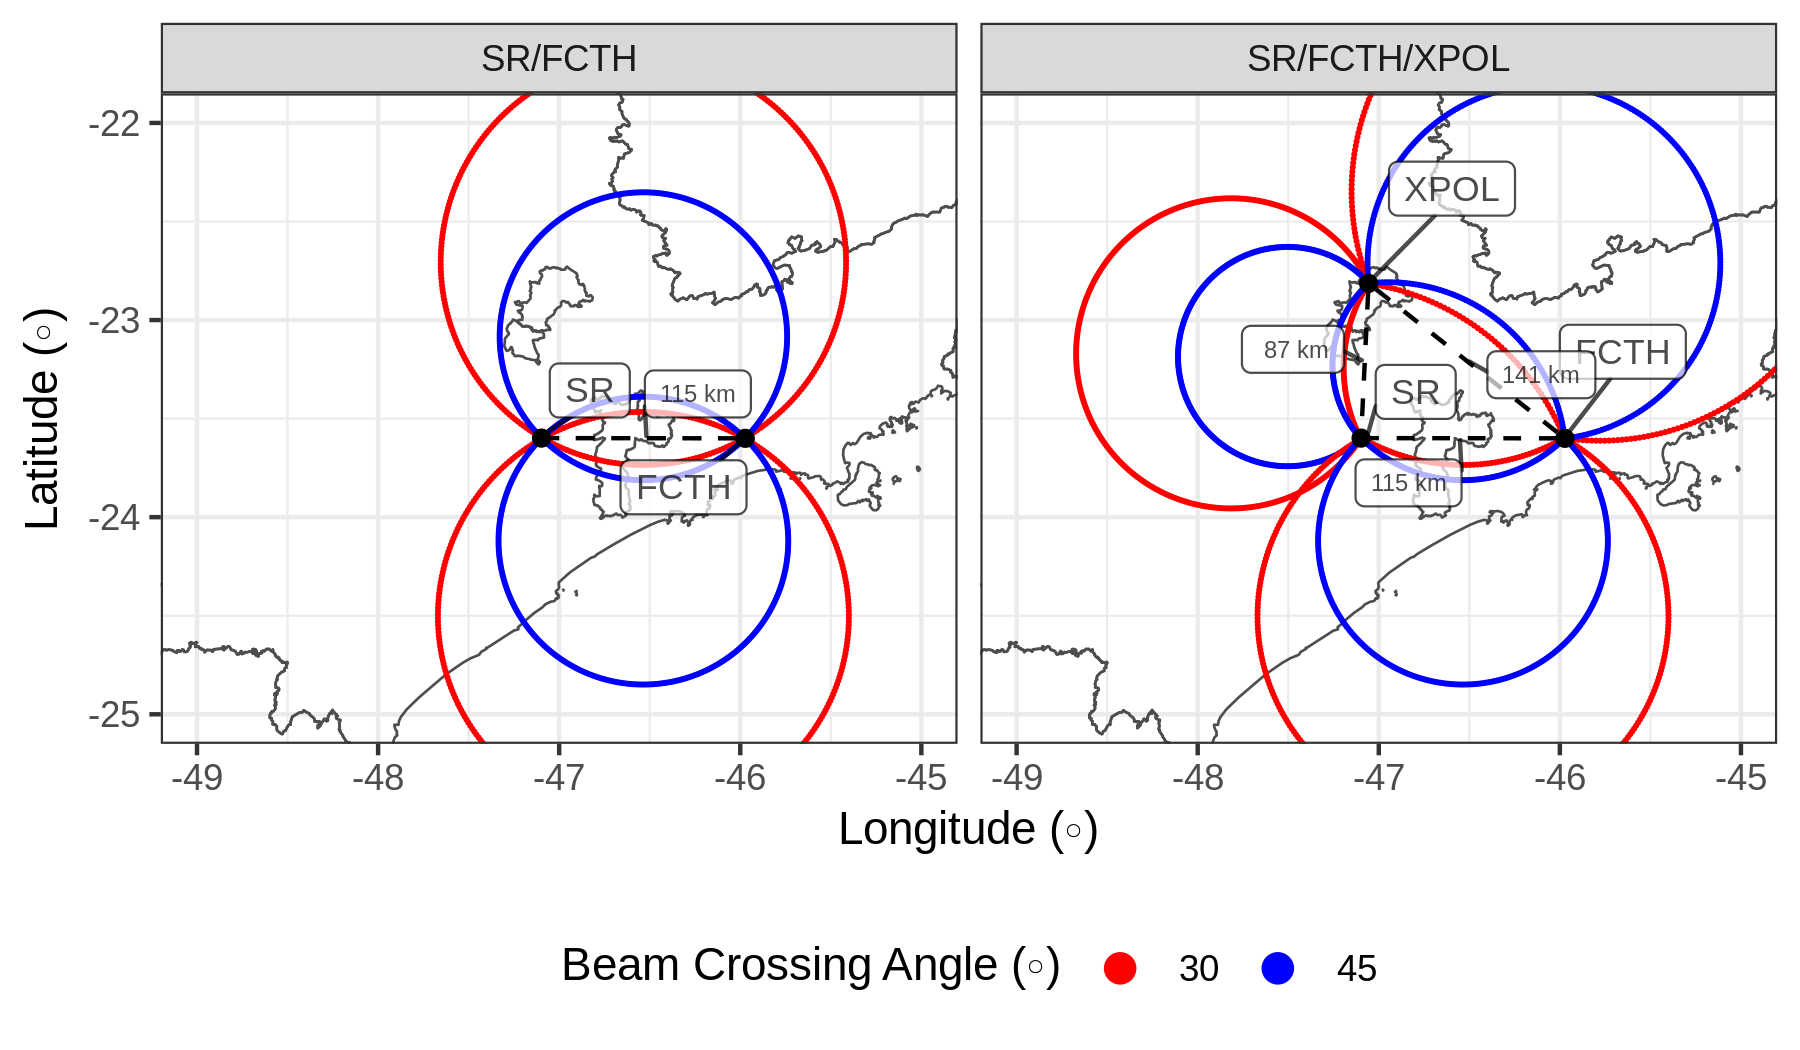
\includegraphics[width=0.65\columnwidth]{../General_Processing/figures/dual_doppler_lobes.png}
		\legend{Fonte: Produzido pela autora.}
	\end{center}
\end{figure}

Para calcular as estimativas de vento usando Dual e Multi-Doppler, o pacote MultiDop \url{https://github.com/nasa/MultiDop} foi utilizado. Desenvolvido em Python e C a partir da metodologia de \citeonline{Shapiro2009} e \citeonline{Potvin2012b} e compatível com o pacote Py-ART \cite{Helmus2016}, este pacote extrai o campo tridimensional de velocidade do vento a partir de uma combinação de 2 ou 3 radares. A metodologia usada nos cálculos é baseada em 3DVAR (\textit{3D Variational Analysis}, Análise Variacional em 3D), em que as componentes cartesianas do vento $u$, $v$ e $w$ são calculadas minimizando uma função custo total $J$ que quantifica erros nas restrições relacionadas aos dados ($J_O$), às equações de conservação de massa ($J_M$) e vorticidade ($J_V$) e à suavização ($J_S$):

\begin{equation}
	J=J_O+J_M+J_V+J_S
\end{equation}

Cada função custo é equivalente ao erro multiplicado por um coeficiente de ajuste $C$, que define o peso que esse erro terá no valor final de velocidade do vento \cite{Potvin2012b}. O pacote MultiDop permite que esses coeficientes sejam definidos pelo usuário - a \autoref{tabela_multidop} mostra os coeficientes escolhidos para as análises, similares a \citeonline{Potvin2012b}, além de outras configurações.

\begin{table}[htb]
	\IBGEtab{%
		\caption{Parâmetros de configuração do MultiDop para cálculos de Dual e Multi-Doppler.}%
		\label{tabela_multidop}
	}{%
		\begin{tabularx}{\textwidth}{YY}
			\toprule
			Resolução da grade & $1 \times 1 \times 1\:km$ \\
			\midrule
			Restrição da conservação de massa & Aproximação anelástica \\
			\midrule 
			Restrição de suavização & Derivadas de segunda ordem \\
			\midrule 
			Pesos na restrição de dados & Pesos iguais para todas as observações \\
			\midrule 
			Condição inicial da tempestade (deslocamento constante) & $U_t = V_t = -10\:ms^{-1}$ \\
			\midrule 
			Impor $w=0$ no topo & Sim \\
			\midrule
			Coeficiente da restrição dos dados & $1$ \\
			\midrule 
			Coeficiente da restrição da equação de continuidade de massa & $30$ \\
			\midrule 
			Coeficiente da restrição da equação de vorticidade & $1e^{-3}$ \\
			\midrule 
			Coeficiente de suavização horizontal & $1e^{-2}$ \\
			\midrule 
			Coeficiente de suavização vertical & $1e^{-2}$ \\
			\midrule
			Coeficiente da restrição da sondagem & $0$ \\
			\midrule 
			Todos os pesos constantes & Sim \\
			\midrule 
			Filtros & Nenhum \\
			\midrule 
			Estatísticas de verificação computadas apenas dentro do domínio de 2+ radares Doppler & Sim \\
			\midrule 
			Critério do domínio & 10 pontos \\
			\midrule
			Altura de corte & $0\:km$ \\
			\midrule 
			Matrizes de cobertura de fundo para ângulos de cruzamento de feixe ótimos para dois radares & Sim para todas as combinações \\
			\midrule 
			Matrizes de cobertura de fundo para ângulos de cruzamento de feixe aceitáveis para dois radares & Sim para todas as combinações \\
			\midrule 
			Matrizes de cobertura de fundo para um radar individual & Não para todos \\
			\midrule 
			Multiplicador do peso dos dados quando todos os radares tem bons ângulos de cruzamento do feixe & $SR=1e^{-3}$, $FCTH=XPOL=1$\\
			\bottomrule
		\end{tabularx}%
	}{%
		\fonte{Produzido pela autora.}%
	}
\end{table}


Como mostrado na \autoref{tabela_multidop}, os dados de radar foram convertidos para uma grade de $1\:x\:1\:x\:1\:km$. Além disso, problemas de ambiguidade da velocidade radial - quando a velocidade radial é maior do que a velocidade de Nyquist (\autoref{nyquist}) - foram corrigidos usando algoritmos baseado na região (analisa os dados por região de velocidades parecidas) e baseado em um esquema em quatro dimensões (4DD, \textit{Four-Dimensional Doppler Dealising Scheme}) \cite{James2001}, ambos presentes no pacote Py-ART; no caso do algoritmo 4DD, uma radiossondagem (novamente da estação do Campo de Marte) foi utilizada como condição inicial. Como forma de complementar as correções automáticas, correções manuais dos dados de velocidade radial foram feitas usando o software Solo3 \url{https://www.eol.ucar.edu/software/solo3}.

\begin{figure}[htb]
	\begin{center}
		\caption{Velocidade radial verdadeira vs medida de um alvo com uma velocidade de Nyquist de $10\:ms^{-1}$ mostrando a ambiguidade para valores de velocidade verdadeira além do intervalo de $-10$ a $10\:ms^{-1}$} 
		\label{nyquist}
		%		\setcaptionmargin{1cm}
		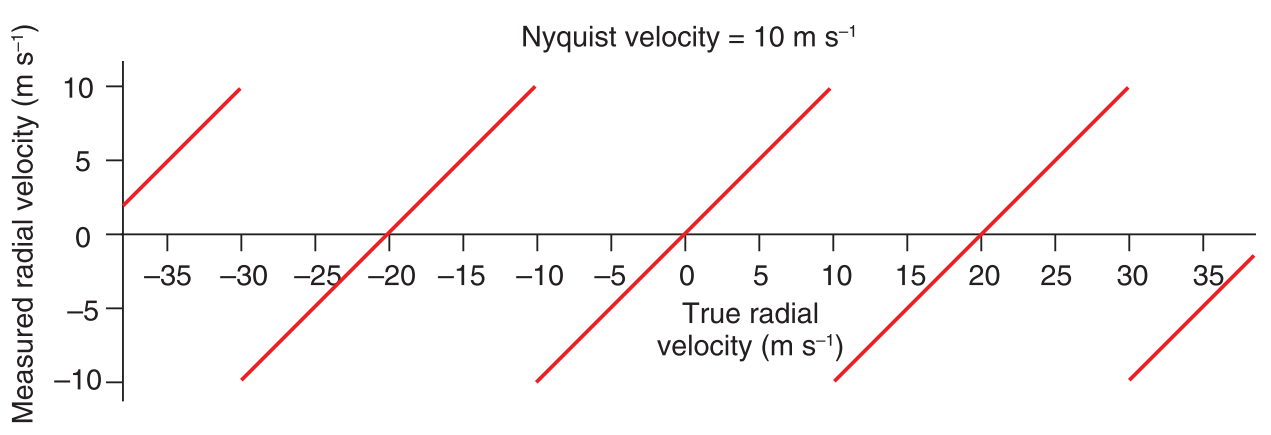
\includegraphics[width=\columnwidth]{figs/nyquist_rauber.png}
		\legend{Fonte: \citeonline{Rauber2018}.}
	\end{center}
\end{figure}

\newpage

\section{Rede de Detecção de Raios}\label{raios}

A atividade elétrica dos casos selecionados foi analisada através dos dados do Sistema Brasileiro de Detecção de Descargas Elétricas (BrasilDAT) \cite{Naccarato2014}. Essa rede opera entre as faixas de frequência LF (\textit{Low Frequency}, Baixa Frequência) e HF (\textit{High Frequency}, Alta Frequência), detectando pulsos eletromagnéticos - chamados de strokes neste trabalho - emitidos pelas descargas elétricas através da técnica do tempo de chegada \cite{Lewis1960}. Devido à larga banda de frequência, é possível diferencial descargas de retorno de raios nuvem-solo (\textit{cloud-to-ground}, CG) e pulsos de raios intranuvem (\textit{intra-cloud}, IC), além de estimar a polaridade dos raios nuvem-solo através do sinal do pico de corrente. A eficiência de detecção estimada da rede é de $60$ a $70\%$ para raios IC e de $95\%$ para raios CG (Dr. Kleber Naccarato, ELAT-CCST-INPE, comunicação pessoal, 2018). Os dados dessa rede foram fornecidos pelo Grupo de Eletricidade Atmosférica (ELAT) do INPE e agrupados em flashes (\autoref{strokestoflashes}).

\subsection{Conversão Strokes-Flashes}\label{strokestoflashes}

Devido ao fato de que strokes estão associados a descargas de retorno e pulsos que não necessariamente representam raios distintos (um raio nuvem-solo, por exemplo, pode ser constituído de diversas descargas de retorno), esses dados foram convertidos em flashes, que representam todo o evento de uma descarga elétrica \cite{MacGorman1998b}. De acordo com \citeonline{Cummins1998} e \citeonline{Murphy2015}, strokes devem ser agrupados em flashes seguindo as seguintes considerações:

\begin{alineas}
	\item Strokes devem ser agrupados em um período total de $1\:s$, com intervalo entre strokes de até $500\:ms$;
	\item Strokes subsequentes devem estar em um raio de até $10\:km$ a partir do primeiro; pode-se considerar strokes subsequentes em um raio de até $50\:km$, desde que esteja dentro do intervalo de $500\:ms$;
	\item A multiplicidade de um flash (quantidade de strokes em um único flash) pode ser de até 63 (1023) strokes CG (IC).
\end{alineas} 

Para fazer o agrupamento seguindo as orientações acima, o algoritmo DBSCAN (\textit{Density-Based Spatial Clustering of Application with Noise}, Agrupamento Espacial Baseado em Densidade de Aplicação com Ruído) de agrupamento de dados foi utilizado. Ele usa a distância entre pontos $\epsilon$ e a quantidade mínima de pontos $min_{pts}$ para agrupar qualquer matriz de dados n-dimensional \cite{Ester1996, Kriegel2011}. \citeonline{Hutchins2014} e \citeonline{Hutchins2014a} usaram este método para agrupar strokes em flashes e em conjuntos de tempestades com raios, e a mesma abordagem foi adotada neste trabalho.

Como o algoritmo DBSCAN usa apenas dois parâmetros ($\epsilon$ e $min_{pts}$), enquanto que o agrupamento de strokes em flashes precisa de três (distância entre pontos $\epsilon_{spc}$, distância temporal $\epsilon_{t}$ e quantidade mínima de pontos $min_{pts}$), duas etapas são necessárias: agrupar os dados em função do tempo (usando $\epsilon_{t}$) e depois agrupar em função do espaço bidimensional (usando $\epsilon_{\text{spc}}$ em latitude e longitude). A partir das orientações de \citeonline{Cummins1998} e \citeonline{Murphy2015} e após alguns testes com $\epsilon_{spc}$ (\refanexo{anexo_conversao}), definiu-se que $min_{pts}=1$, $\epsilon_{t}=0,5\:s$ e $\epsilon_{spc}=2,5\:km$. O algoritmo foi implementado e adaptado usando a linguagem R.

A \autoref{flash_stats} mostra as características dos dados de flashes gerados usando as especificações acima. É possível observar que a distribuição de tempos entre strokes e entre flashes (\autoref{flash_stats}a) apresentam picos em aproximadamente $0,1$ e $1\:s$, respectivamente; o tempo máximo entre strokes é de aproximadamente $500\:ms$, compatível com \citeonline{Cummins1998}. A maioria dos dados apresentou um stroke por flash (\autoref{flash_stats}b), com registros de até 17 strokes por flash, compatível com \citeonline{Murphy2015}. A distribuição espacial de distância entre strokes em um flash (\autoref{flash_stats}c) possui maior concentração de dados dentro do intervalo de 0 a $2,5\:km$ de latitude e longitude, com distâncias de até 7 km, também compatível com \citeonline{Cummins1998}. Assim, pode-se dizer que o algoritmo de agrupamento de strokes em flashes foi bem sucedido em agrupar os dados dentro das orientações citadas.

\begin{figure}[htb]
	\begin{center}
		\caption{Histogramas de tempo entre strokes e entre flashes (a), número de strokes por flash (b) e distância latitude e longitudinal entre strokes em um flash (c)} 
		\label{flash_stats}
		%		\setcaptionmargin{1cm}
		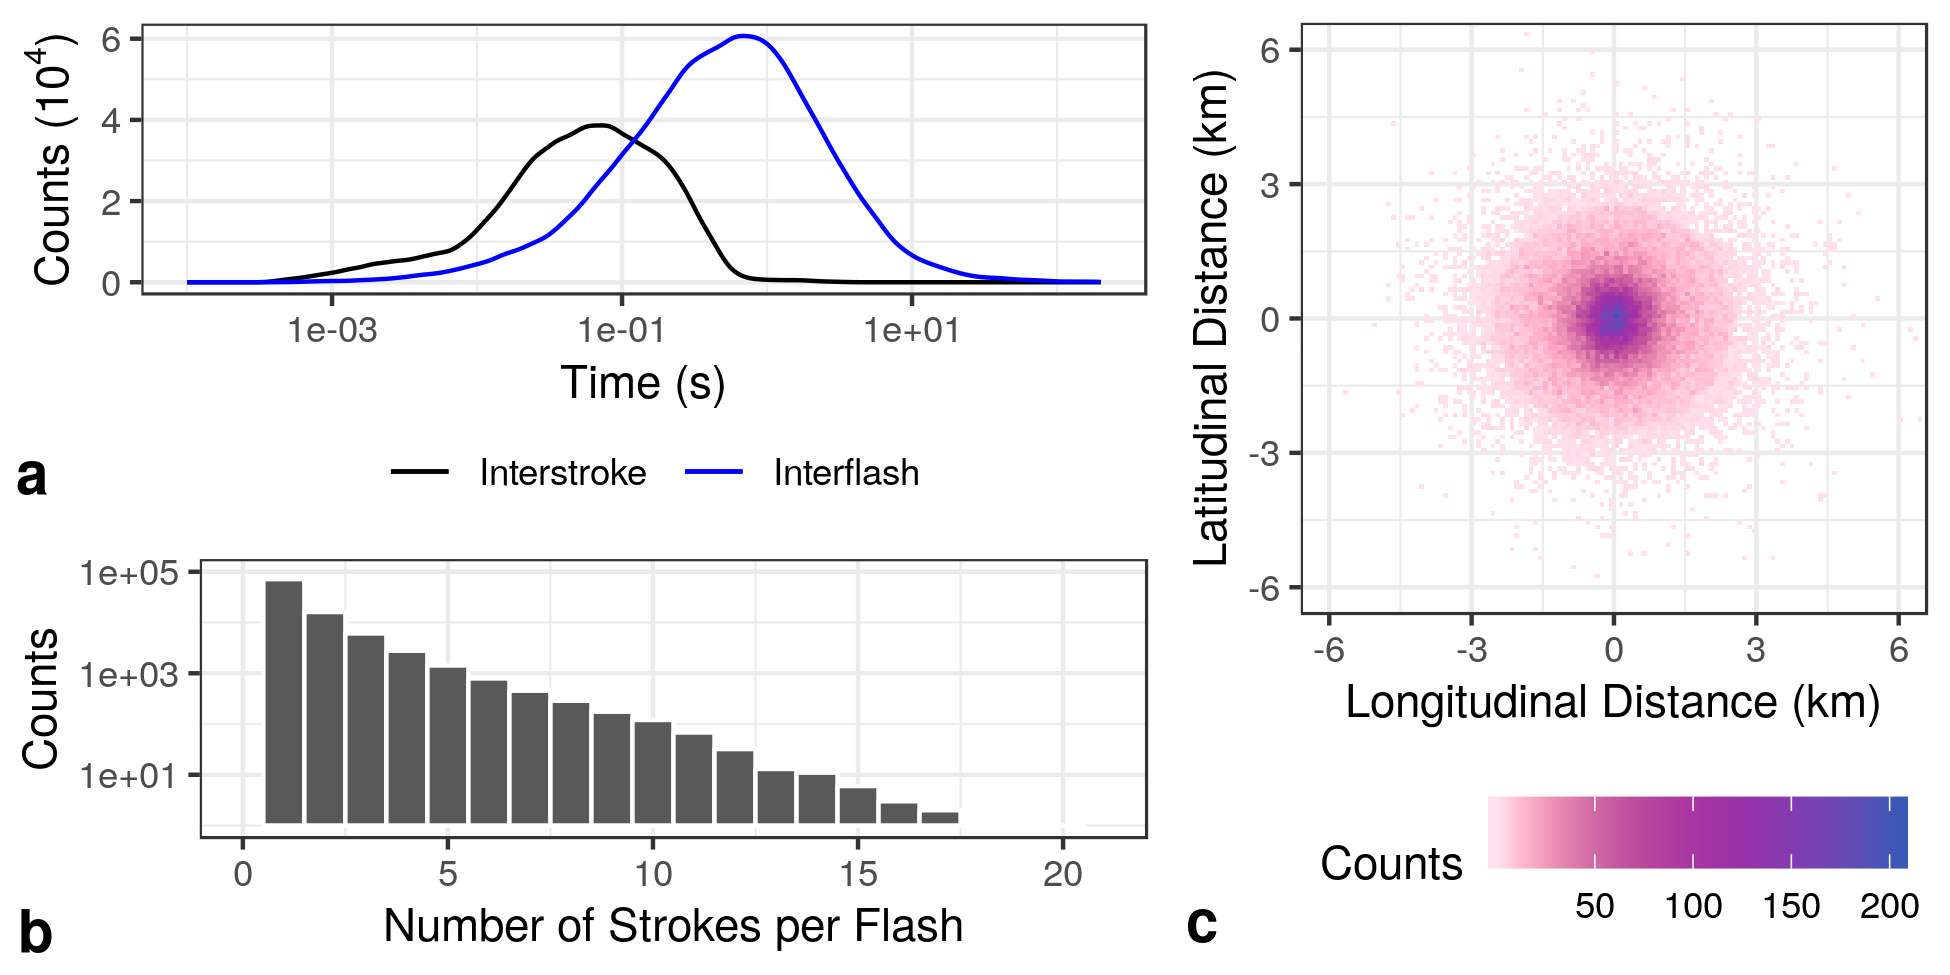
\includegraphics[width=\columnwidth]{../Lightning_Processing/figures/brasildat_flash_stats.png}
		\legend{Fonte: Produzido pela autora.}
	\end{center}
\end{figure}

\section{Outras Bases de Dados}\label{outros_dados}

Para analisar o ambiente sinótico associado a cada caso, dados da reanálise ERA5 e do satélite GOES-16 foram utilizados, descritos a seguir.

\subsection{Reanálise} \label{era5}

O conjunto de dados de reanálise ERA5 \cite{Copernicus2017} é desenvolvido pelo ECMWF (\textit{European Centre for Medium-Range Weather Forecasts}, Centro Europeu para Previsões de Tempo de Médio Alcance) e estão disponíveis publicamente para o período de 2010 a 2-3 meses antes do presente. Este modelo eventualmente substituirá o conjunto de reanálise mais antigo ERA-Interim. A resolução espacial destes dados é de $30\:km$ de cobertura global e 137 níveis verticais, da superfície até $80\:km$ de altura; a resolução temporal é de $1\:h$. Foram usados campos de pressão em superfície, geopotencial, vento e CAPE em diferentes níveis de pressão. Os dados foram obtidos a partir do Armazenamento de Dados Climáticos (\textit{Climate Data Store}, CDS) do Serviço de Mudanças Climáticas Copernicus (\textit{Copernicus Climate Change Service}, CCCS) do ECMWF e processados usando a linguagem Python.

\subsection{Satélite} \label{goes16}

O satélite GOES-16 foi lançado em dezembro de 2016 e está operacional desde 18 de dezembro de 2017. Ele possui 16 canais no principal sensor (ABI - \textit{Advanced Baseline Imager}, Imageador Avançado de Base), além de sensores de raios (GLM - \textit{Geostationary Lightning Mapper}, Mapeador Geoestacionário de Raios) e que medem atividade solar. O modo de escaneamento \textit{Full Disk} (Disco Inteiro) gera uma imagem que inclui a América do Sul continuamente com uma resolução temporal de 5 a 15 minutos e espacial de 0,5 a $2\:km$. Considerando o período de estudo (\autoref{tabela_casos}), 3 dos 5 casos foram analisados com estes dados, usando o canal 13 do ABI, chamado de \textit{"clean"\ longwave infrared window} (janela "limpa" do infravermelho de onda longa), para identificar os sistemas mais intensos e profundos (menor temperatura de brilho). Os dados de nível 2 (convertidos em uma grade latitude-longitudinal e que servem como base para os cálculos de produtos derivados de combinação dos canais) foram obtidos do repositório da NOAA (\textit{National Oceanic and Atmospheric Administration}, Administração Nacional Oceânica e Atmosférica) na AWS (\textit{Amazon Web Services}, Serviços Web da Amazon) \url{https://docs.opendata.aws/noaa-goes16/cics-readme.html} e processados usando a linguagem Python.